% -----------------------------------------------
% Template for ISMIR Papers
% 2019 version, based on previous ISMIR templates

% Requirements :
% * 6+n page length maximum
% * 4MB maximum file size
% * Copyright note must appear in the bottom left corner of first page
% * Clearer statement about citing own work in anonymized submission
% (see conference website for additional details)
% -----------------------------------------------

\documentclass{article}
\usepackage[T1]{fontenc} % add special characters (e.g., umlaute)
\usepackage[utf8]{inputenc} % set utf-8 as default input encoding
\usepackage{ismir,amsmath,cite,url}
\usepackage{graphicx}
\usepackage{color}

% Optional: To use hyperref, uncomment the following.
% \usepackage[bookmarks=false,hidelinks]{hyperref}
% Mind the bookmarks=false option; bookmarks are incompatible with ismir.sty.

\newcommand{\setName}{Fourier}

% Title.
% ------
\title{The \setName~Set: Beats, Downbeats, and Functional Segment Annotations of Western Popular Music}

% Note: Please do NOT use \thanks or a \footnote in any of the author markup

% Single address
% To use with only one author or several with the same address
% ---------------
%\oneauthor
% {Names should be omitted for double-blind reviewing}
% {Affiliations should be omitted for double-blind reviewing}

% Two addresses
% --------------
%\twoauthors
%  {First author} {School \\ Department}
%  {Second author} {Company \\ Address}

%% To make customize author list in Creative Common license, uncomment and customize the next line
%  \def\authorname{First Author, Second Author}


% Three addresses
% --------------
\threeauthors
  {First Author} {Affiliation1 \\ {\tt author1@ismir.edu}}
  {Second Author} {\bf Retain these fake authors in\\\bf submission to preserve the formatting}
  {Third Author} {Affiliation3 \\ {\tt author3@ismir.edu}}

%% To make customize author list in Creative Common license, uncomment and customize the next line
%  \def\authorname{First Author, Second Author, Third Author}

% Four or more addresses
% OR alternative format for large number of co-authors
% ------------
%\multauthor
%{First author$^1$ \hspace{1cm} Second author$^1$ \hspace{1cm} Third author$^2$} { \bfseries{Fourth author$^3$ \hspace{1cm} Fifth author$^2$ \hspace{1cm} Sixth author$^1$}\\
%  $^1$ Department of Computer Science, University , Country\\
%$^2$ International Laboratories, City, Country\\
%$^3$  Company, Address\\
%{\tt\small CorrespondenceAuthor@ismir.edu, PossibleOtherAuthor@ismir.edu}
%}
%\def\authorname{First author, Second author, Third author, Fourth author, Fifth author, Sixth author}


\sloppy % please retain sloppy command for improved formatting

\begin{document}

%
\maketitle
%
\begin{abstract}
    We introduce the \setName\footnote{Temporary name for the blind review process.}~set: a collection of annotations of beats, downbeats, and functional segmentation for over 700 tracks that covers a wide range of western popular music.
    Given the variety of annotated music information types in this set, and how strongly these three types of data are typically intertwined, we believe it could potentially foster research that focuses on multiple retrieval tasks at once.
    The dataset includes additional metadata such as MusicBrainz identifiers to support the linking of the dataset to third-party information or audio data when available.
    We describe the methodology employed in acquiring this set, including the annotation process and song selection. 
    In addition an initial data exploration of the annotations and actual dataset content is conducted. 
    Finally, we provide a series of baselines of the \setName~set with standard beat-trackers, downbeat predictors, and structural segmentation algorithms in the literature.
\end{abstract}
%
\section{Introduction}\label{sec:introduction}

The tasks of beat detection, downbeat prediction, and structural segmentation constitute a fundamental part of the field of MIR.
These three musical characteristics are often related: downbeats define the first beat of a given music measure, and long structural music segments tend to begin and end on specific beat locations --frequently on downbeats.
The automatic estimation of such information could result in better musical systems such as more accurate automatic DJ-ing, better intra- and inter-song navigation, further musicological insights of large collections, \emph{etc}.
While several approaches exploiting more than one of these musical traits have been proposed~\cite{Bock2016, Fuentes2019}, the lack of human annotated data containing the three of them for a single collection are scarce.
This limits the amount of potential of certain methods, especially those that require large amounts of information (e.g., deep learning~\cite{Humphrey2012}).

In this paper we present the \setName~set: human annotations of beats, downbeats, and functional segmentation for over 700 tracks of western popular music.
These annotations were gathered with the aim of having a significant amount of data to train models to improve the prediction of such musical attributes, which would later be applied to various products offered by \setName.
By releasing this set to the public, it is our aim to let the research community explore and exploit these annotations to advance the tasks of beat tracking, downbeat prediction, and automatic functional structural segmentation.
We discuss the methodology to acquire these data, including the song selection process, and the inclusion of standard identifiers (Acoustid and MusicBrainz) and onsets for the first 30 seconds of the tracks to allow for other researchers to more easily access and align, when needed, the actual audio content.
Furthermore, we present a series of results with standard algorithmic approaches in the literature with the goal of having an initial public benchmark of this set.

The rest of this work is organized as follows: Section~\ref{sec:background} contains a review of the most relevant public datasets of the tasks at hand; Section~\ref{sec:dataset} discusses the actual \setName~set, including the data gathering, their formatting, and various statistics; Section~\ref{sec:results} presents various benchmarks in the set; and Section~\ref{sec:conclusions} draws some final conclusions and discloses future remarks.
%
\section{Background}\label{sec:background}

In this section we discuss previously published datasets, and break them down based on the type of information they provide.

Beats datasets.

Downbeat datasets.

Segmentation datasets: SALAMI~\cite{Smith2011}.

Combined datasets: The Beatles Dataset~\cite{Mauch2009a}.

\section{The \setName~Set}\label{sec:dataset}

Explanation of dataset.\footnote{URL not displayed for the blind review process.}

\subsection{Data Gathering}

How were the songs selected. Show genre distribution plot.

Who annotated them (e.g., professional musicians?)

How they annotated them (tools, revisions, etc.). Why only flat segmentation.

Why were the songs selected (motivation behind \setName).

Additional data could be obtained by data augmentation~\cite{Mcfee2015}.

\subsection{Data Formatting}

JAMS~\cite{Humphrey2014}.

MusicBrainz IDs.

Acoustid IDs.

Train/Test splits.

\subsection{Data Statistics}

Show plots and statistics for: 

\subsubsection{beats}

\subsubsection{downbeats}

\subsubsection{segmentation}

How many segments start/end on downbeats?

\section{Results}\label{sec:results}

\subsection{Beat Results}

Beat results

\subsection{Downbeat Results}

Downbeat results

\subsection{Segmentation Results}

Segmentation results. Using~\cite{Nieto2016}. Serr\`a algorithm~\cite{Serra2014}. Results included in CVS format for all dataset.

\begin{figure}
    \centerline{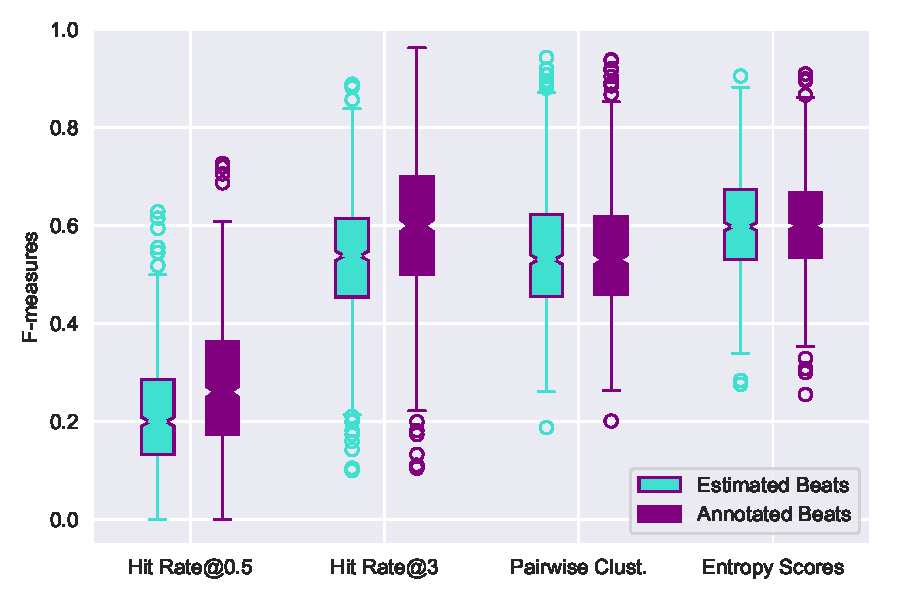
\includegraphics[width=\columnwidth]{figs/segment_results.pdf}}
    \caption{Segmentation results}
    \label{fig:segment_results}
\end{figure}

\subsection{Beat + Segmentation Results}

Beat + Segmentation.

\section{Conclusions}\label{sec:conclusions}

Potential of combined data + large amounts of annotations.

% For bibtex users:
\bibliography{ISMIRtemplate}

\end{document}
